\documentclass[10pt,twocolumn,letterpaper]{article}

\usepackage{cvpr}
\usepackage{times}
\usepackage{epsfig}
\usepackage{graphicx}
\usepackage{amsmath}
\usepackage{amssymb}
\usepackage{subfigure}

% Include other packages here, before hyperref.

% If you comment hyperref and then uncomment it, you should delete
% egpaper.aux before re-running latex.  (Or just hit 'q' on the first latex
% run, let it finish, and you should be clear).
\usepackage[pagebackref=true,breaklinks=true,letterpaper=true,colorlinks,bookmarks=false]{hyperref}

% \cvprfinalcopy % *** Uncomment this line for the final submission

\def\cvprPaperID{****} % *** Enter the CVPR Paper ID here
\def\httilde{\mbox{\tt\raisebox{-.5ex}{\symbol{126}}}}

% Pages are numbered in submission mode, and unnumbered in camera-ready
\ifcvprfinal\pagestyle{empty}\fi
\begin{document}

%%%%%%%%% TITLE
\title{Multilayer Coupled Orthogonal Dictionary Learning for Robust Real Image Denoising}

\author{First Author\\
Institution1\\
Institution1 address\\
{\tt\small firstauthor@i1.org}
% For a paper whose authors are all at the same institution,
% omit the following lines up until the closing ``}''.
% Additional authors and addresses can be added with ``\and'',
% just like the second author.
% To save space, use either the email address or home page, not both
\and
Second Author\\
Institution2\\
First line of institution2 address\\
{\tt\small secondauthor@i2.org}
}

\maketitle
%\thispagestyle{empty}

%%%%%%%%% ABSTRACT
\begin{abstract}
Existing image denoising methods largely depends on noise modeling and estimation. The commonly used noise models, additive white Gaussian or Mixture of Gaussians, are inflexible in describing the complex noise on real noisy images or time consuming in parametric estimation, respectively. Therefore, how to perform image denoising \textbf{without} noise modeling and estimation is an essential while challenging problem. In this paper, we attempt to solve this problem by directly learning the transformation process between the noisy images and clean ones. The transformation is learned on patches instead of images for dimensional tractability. The learning data is collected by constructing paired noisy and clean patches from unpaired real noisy and clean images. Since real noise is signal dependent and from several main sources \cite{healey1994radiometric}, we cluster the learning data into multiple components. For each component, we learn in an integrated way two paired dictionaries for the noisy and clean data and two transformation functions between them. The overall learned transformation process could remove the noise from different sources. Experiments show that the proposed Paired Dictionary and Transformation Learing (PDTL) model achieves better performance on denoising real noisy images than other noise estimation based methods.
\end{abstract}

%%%%%%%%% BODY TEXT
\section{Introduction}
Image denoising is a fundermental problem in computer vision and image processing. It is an ideal platform for testing natural image models and provides high-quality images for other conputer vision tasks such as image registration, segmentation, and pattern recognition, etc. For several decades, there emerge numerous image denoising methods \cite{nlm,foe,ksvd,bm3d,lssc,epll,burger2012image,wnnm,csf,pgpd,chen2015learning,fullyblind,rabie2005robust,Liu2008,almapg,noiseclinic,Zhu_2016_CVPR,crosschannel2016}, and most of them focus on dealing with additive white Gaussian noise (AWGN). Among these methods, \cite{fullyblind,rabie2005robust,Liu2008,almapg,noiseclinic,Zhu_2016_CVPR,crosschannel2016} are designed to deal with real noisy images. Almost all these methods coincidently employ a two-stage framework: in the first stage, assuming a distribution model (usually Gaussian) on the noise and estimate its parameters; in the second stage, performing denoising with the help of the noise modeling and estimation in the first stage. However, the Gaussian assumption is inflexible in describing the complex noise on real noisy images \cite{Liu2008,crosschannel2016}. Although the mixture of Gaussians (MoG) model is possible to approximate any unknown noise \cite{Zhu_2016_CVPR}, estimating its parameters is often time consuming via nonparametric Bayesian techniques \cite{Zhu_2016_CVPR} \cite{Bishop}. To avoid the above mentioned problems, it is naturally to ask, whether it is possible to perform denoising on real noisy images without noise modeling and estimation? 

To answer this question, we look close into several discriminative learning methods \cite{burger2012image,csf,chen2015learning} achieving expressive performance on Gaussian noise removal. These methods require a set of paired images, namely clean ground-truth images and the simulated noisy counterparts degraded by identical noise (mainly additive white Gaussian noise, AWGN), to learn an effective model for image denoising. However, the noise in real images are much more complex than Gaussian, since it depends on camera series, brands, as well as the settings (ISO, shutter speed, and aperture, etc). Thus, the model learned with AWGN would become much less effective for denoising real noisy images. What's more, usually real noisy images do not have clean counterparts. Therefore, almost all current discriminative learning methods cannot be directly applied to real noisy images.

The above mentioned limitations indicate that, novel denoising methods are been waiting for which can: 1) avoid noise modeling and estimation; 2) learn without paired training images; 3) deal with complex noise on real noisy images. In this paper, we attempt to solve the three problems in an integrated way for robust real image denoising. Specifically, we collect a comprehensive set of real noisy images and an independent set of clean images, and propose a learning based model to directly transform the noisy input into clean counterparts. The rationale is that, the noise on real noisy images obtained through in-camera imaging pipeline \cite{NewInCamera} are structure dependent \cite{crosschannel2016} and identified by several main types \cite{healey1994radiometric,tsin2001statistical}. To better deal with different stuctures and noise sources, we propose to learn our model on multile clusters of image patches instead of on a set of large images. Besides, it is difficult to learn models on whole images since that natural images are of high dimensionality. What's more, for our learning model, though images are different, it is possible to find a cluster of patches in clean images which are similar to given noisy patches. For each cluster of patches, we learn two dictionaries and transformation functions to characterize the structures of and relationship between niosy and clean image patches. We perform comprehensive experiments on real noisy images captured by different CMOS or CCS sensors. The results demonstrate that our method achieves comparable or even better performance on denoising real noisy images. This reveals the potential advantages of 
dscriminative learning methods on robust and complex real noisy image denoising problem.

%The in-camera imaging pipeline usually includes image demosaicing, white balance and color space transform, gamut mapping, tone mapping, and JPEG comression \cite{NewInCamera,crosschannel2016}.

\subsection{Our Contributions}
The contributions of this paper are closely related to the three problems we mentioned above, and summarized as follows:
\begin{itemize}
\item To avoid noise modeling and estimation, we propose a noval learning based model which directly transform noisy images into clean conuterparts;
\item To learn without paired training images, we perform the learning on paired image patches extracted from unpaired noisy and clean images;
\item To deal with different structures and nise sources, we employ a "divide-and-coquer" strategy on the training data, and for each paired cluster of similar patches, we learn two dictionaries and transformation function for noisy and clean data;
\item The proposed method achieves better performance than other competing methdos on real noisy image denoising problem.
\end{itemize}

\section{Related Work}
\subsection{Couple dictionary learning}
Coupled dictionary learning (CDL) is a frequently used learning framework for cross-style image synthesis problems, such as image super-resolution, photo-sketch synthesis. CDL aims at learning a pair of dictionaries as well as the relationships between the two cross-domain image styles. Hence, the information from the source image style can be applied to synthesize the image at the target style. The relationships are often assumed to be identical mapping (coupled) \cite{yang2010image}, linear mapping (semi-coupled) \cite{wang2012semi}. Yang et al. \cite{yang2010image} assumed that LR image patches have the same sparse representations as their HR versions do, and proposed a joint dictionary learning model for SR using concatenated HR/LR image features. They later imposed relaxed constraints on the observed dictionary/coefficient pairs across image domains for improved performance. Wang et al. \cite{wang2012semi} further proposed a semi-coupled dictionary
learning (SCDL) scheme by advancing a linear mapping for cross-domain image sparse representation. Their method
has been successfully applied to applications of image SR and cross-style synthesis.

\subsection{Real Image Denoising}
To the best of our knowledge, the study of real image denoising can be dated back to the BLS-GSM model \cite{blsgsm}, in which Portilla et al. proposed to use scale mixture of Gaussian in overcomplete oriented pyramids to estimate the latent clean images. In \cite{fullyblind}, Portilla proposed to use a correlated Gaussian model for noise estimation of each wavelet subband. Based on the robust statistics theory \cite{huber2011robust}, the work of Rabie \cite{rabie2005robust} modeled the noisy pixels as outliers, which could be removed via Lorentzian robust estimator. In \cite{Liu2008}, Liu et al. proposed to use 'noise level function' (NLF) to estimate the noise and then use Gaussian conditional random field to obtain the latent clean image. Recently, Gong et al. proposed an optimization based method \cite{almapg}, which models the data fitting term by weighted sum of $\ell_{1}$ and $\ell_{2}$ norms and the regularization term by sparsity prior in the wavelet transform domain. Later, Lebrun el al. proposed a multiscale denoising algorithm called 'Noise Clinic' \cite{noiseclinic} for real image denoising task. This method generalizes the NL-Bayes \cite{nlbayes} to deal with signal, scale, and frequency dependent noise. Recently, Zhu et al. proposed a Bayesian model \cite{Zhu_2016_CVPR} which approximates the noise via Mixture of Gaussian (MoG) model \cite{Bishop}. The clean image is recovered from the noisy image by the proposed Low Rank MoG filter (LR-MoG). However, noise level estimation is already a challenging problem and denoising methods are quite sensitive to this parameter. Moreover, these methods are based on shrinkage models that are too simple to reflect reality, which results in over-smoothing of important structures such as small-scale text and textures. 

\section{Double Semi-Couple Dictionary Learning}
In this section, we first formulate the real image denoising problem from the perspective of learning based model and then provide the optimization for the problem.
\subsection{Problem Formulation}
For real image denoising, we first collect clean natural images and real noisy images for training. Assume the $\mathbf{X}$ and $\mathbf{Y}$ are unpaired clean image patches and real noisy patches. Let the $\mathbf{X} = \mathbf{D}_{x}\mathbf{A}_{x}$ and $\mathbf{Y} = \mathbf{D}_{y}\mathbf{A}_{y}+\mathbf{V}_{y}$, where $\mathbf{V}_{y}$ is the real noise of which we don't know the distribution. 
\begin{equation}
\begin{split}
&\min_{\mathbf{D}_{x},\mathbf{D}_{y},\mathbf{A}_{x},\mathbf{A}_{y}}
\emph{E}_{data}(\mathbf{X},\mathbf{D}_{x},\mathbf{A}_{x})+
\emph{E}_{data}(\mathbf{Y},\mathbf{D}_{y},\mathbf{A}_{y},\mathbf{V}_{y})
\\
&
+\emph{E}_{map}(f_{1}(\mathbf{A}_{x}),f_{2}(\mathbf{A}_{y}))+
\emph{E}_{reg}(\mathbf{A}_{x},\mathbf{A}_{y},f_{1},f_{2},\mathbf{D}_{x},\mathbf{D}_{y},\mathbf{V}_{y})
\end{split}
\end{equation}

This framework doesn't need noise modeling and estimation. However, we still model the noise by $\mathbf{V}_{y}$ for visualization what we have removed during training. The regularization of the noise by $\|\mathbf{V}_{y}\|_{p}^{p}$ can be flexible, that we can penalize it by Frobenius norm, $\ell_{1}$ norm, or any other norms. We employ Frobenius norm here for modeling simplicity. To model the relationship between the representational coefficients, we propose to use two inversible mapping function $f_{1}$ and $f_{2}$. To measure the error, we employ a penalty function $\emph{F}$.
\begin{equation}
\begin{split}
\min_{\mathbf{D}_{x},\mathbf{D}_{y},\mathbf{A}_{x},\mathbf{A}_{y},\mathbf{U}_{x},\mathbf{U}_{y},\mathbf{V}_{y}}
\|\mathbf{X}-\mathbf{D}_{x}\mathbf{A}_{x}\|_{F}^{2}&
\\
+
\|\mathbf{Y}-\mathbf{D}_{y}\mathbf{A}_{y}-\mathbf{V}_{y}\|_{F}^{2}
+
\alpha
\emph{F}(f_{1}(\mathbf{A}_{x}),f_{2}(\mathbf{A}_{y}))&
\\
+
\beta_{x1}\|\mathbf{A}_{x}\|_{1}
+
\beta_{x2}\|\mathbf{A}_{x}\|_{F}^{2}
+
\beta_{y1}\|\mathbf{A}_{y}\|_{1}
+
\beta_{y2}\|\mathbf{A}_{y}\|_{F}^{2}
&
\\
(+
\gamma_{y}\|\mathbf{V}_{y}\|_{p}^{p})
\\
\text{s.t.}
\quad
\|\mathbf{d}_{x,i}\|_{2}=1
, 
\|\mathbf{d}_{y,i}\|_{2}=1
,
\forall{i}
.
\end{split}
\end{equation}
Here, we want to discuss more on the mapping functions $f_{1}, f_{2}$ and the measure function $\emph{F}$. The mapping function can be linear or nonlinear transformations. The linear function can be defined as a mapping matrix $f_{1}(\mathbf{A}_{x})=\mathbf{U}_{x}\mathbf{A}_{x}$ and $f_{2}(\mathbf{A}_{y})=\mathbf{U}_{y}\mathbf{A}_{y}$. The corresponding penalty terms on the mapping matrices are $\|\mathbf{U}_{x}\|_{F}^{2}$ and $\|\mathbf{U}_{y}\|_{F}^{2}$. The nonlinear function can be defined as sigmoid function $f_{1}(\mathbf{A}_{x})=1/(1+\exp\{-\mathbf{A}_{y}\})$. We can also employ "first-linear-then-nonlinear" or "first-nonlinear-then-linear" strategies. Here, we don't have explict penalty terms for the nonlinear mapping functions. The derivatives of the nonlinear case also need further discussions since it is not easy to obtain closed-form solutions with sigmoid functions. In this paper, we utilize linear transformation matrices as the mapping functions $f_{1}$ and $f_{2}$. The measure penalty function is simply defined by Frobenius norm. Hence, the term is defined as $\|\mathbf{U}_{x}\mathbf{A}_{x}-\mathbf{U}_{y}\mathbf{A}_{y}\|_{F}^{2}$. However, this would generate a trivial solution of $\mathbf{U}_{x}=\mathbf{U}_{y}=\mathbf{0}$. In order to avoid this case, we propose to use the inverse of the mapping matrices, i.e., $\mathbf{U}_{x}^{-1}$ and $\mathbf{U}_{y}^{-1}$.

In summary, we propose a Doubly Inversible and Semi-Coupled Dictionary Learing (DISCDL) model to learn the dictionaries and mapping functions between real noisy images and latent clean natural images. 
\begin{equation}
\begin{split}
\min_{\mathbf{D}_{x},\mathbf{D}_{y},\mathbf{A}_{x},\mathbf{A}_{y},\mathbf{U}_{x},\mathbf{U}_{y},\mathbf{V}_{y}}
\|\mathbf{X}-\mathbf{D}_{x}\mathbf{A}_{x}\|_{F}^{2}&
\\
+
\|\mathbf{Y}-\mathbf{D}_{y}\mathbf{A}_{y}-\mathbf{V}_{y}\|_{F}^{2}
+
\alpha
\|\mathbf{U}_{x}^{-1}\mathbf{A}_{x}-\mathbf{U}_{y}^{-1}\mathbf{A}_{y}\|_{F}^{2}&
\\
+
\beta_{x1}\|\mathbf{A}_{x}\|_{1}
+
\beta_{x2}\|\mathbf{A}_{x}\|_{F}^{2}
+
\beta_{y1}\|\mathbf{A}_{y}\|_{1}
+
\beta_{y2}\|\mathbf{A}_{y}\|_{F}^{2}
&
\\
(+
\gamma_{y}\|\mathbf{V}_{y}\|_{p}^{p})
&
\\
+
\lambda_{x}\|\mathbf{U}_{x}^{-1}\|_{F}^{2}
+
\lambda_{y}\|\mathbf{U}_{y}^{-1}\|_{F}^{2}
\\
\text{s.t.}\quad \|\mathbf{d}_{x,i}\|_{2}=1, \|\mathbf{d}_{y,i}\|_{2}=1, \forall{i}.
\end{split}
\end{equation}
This model has three major differences when compared with SCDL model.
\begin{itemize}
\item We use a matrix $\mathbf{V}_{y}$ to model the noise, and we don't set any prior distribution on it. This term can help us visualize the noise we learned from the data, i.e., the real noisy images. This make our model fully data-driven. Since our assumption (we have no assumption at all) on noise is more flexible than others', the noise we obtain in our model can be more accurate than other statistical models such as Gaussian or Mixture of Gaussians. Besides, it is time-consuming to fit the noise model from the online data. 
\item We use two inversible matrices as the mapping transformations between the coefficients of the real noisy patches and the latent clean patches. This makes our model more flexible than SCDL in which the mapping matrix not explictly inversible. Besides, the SCDL can only transform LR images into HG images while our model can transform two different image styles in both direction.
\item The constraints on dictionary atoms in our model is strictly $\|\mathbf{d}_{x,i}\|_{2}=1, \|\mathbf{d}_{y,i}\|_{2}=1$ while the CDL model and SCDL model are $\|\mathbf{d}_{x,i}\|_{2}\le1, \|\mathbf{d}_{y,i}\|_{2}\le1$. This makes our model more robust on the dictionary learning since both the dictionary atoms and sparse coefficients are interacted with each other. The $\le1$ constraints would like to make the coefficients larger and dictionary atoms smaller or even vanish. However, in the training stage, we care more about the dictionary atoms and would rather ignore the sparse coefficients.  
\end{itemize}

\subsection{Model Optimization}
While the objective function in (3) is not convex, it is convex with each varible when other variables are fixed. We employ alternating direction method of multipliers (ADMM) algorithm here. Specifically, we divide the objective function into four sub-problems: 1) updating the sparse coefficients $\mathbf{A}_{x}, \mathbf{A}_{y}$; 2) updating the normalized dictionaries $\mathbf{D}_{x}, \mathbf{D}_{y}$; 3) updating the noise matrix $\mathbf{V}_{y}$; 4) updating the mapping matirces $\mathbf{U}_{x}, \mathbf{U}_{y}$. We discuss the four steps as follows.

\subsubsection{Updating $\mathbf{A}_{x}$ and $\mathbf{A}_{y}$}

\begin{equation}
\begin{split}
\min_{\mathbf{A}_{x}}
\|\mathbf{X}-\mathbf{D}_{x}\mathbf{A}_{x}\|_{F}^{2}
+
\alpha
\|\mathbf{U}_{x}^{-1}\mathbf{A}_{x}-\mathbf{U}_{y}^{-1}\mathbf{A}_{y}\|_{F}^{2}
&
\\
+
\beta_{x1}\|\mathbf{A}_{x}\|_{1}
+
\beta_{x2}\|\mathbf{A}_{x}\|_{F}^{2},
\end{split}
\end{equation}
\begin{equation}
\begin{split}
\min_{\mathbf{A}_{y}}
\|\mathbf{Y}-\mathbf{D}_{y}\mathbf{A}_{y}-\mathbf{V}_{y}\|_{F}^{2}
&
\\
+
\alpha
\|\mathbf{U}_{x}^{-1}\mathbf{A}_{x}-\mathbf{U}_{y}^{-1}\mathbf{A}_{y}\|_{F}^{2}
+
\beta_{y1}\|\mathbf{A}_{y}\|_{1}
+
\beta_{y2}\|\mathbf{A}_{y}\|_{F}^{2}.
\end{split}
\end{equation}

Take $\mathbf{A}_{x}$ as an example, the first and second terms above can be combined to form a new optimization problems as follows:
\begin{equation}
\min_{\mathbf{A}_{x}}
\|\widetilde{\mathbf{X}}-\widetilde{\mathbf{D}}_{x}\mathbf{A}_{x}\|_{F}^{2}
+
\beta_{x1}\|\mathbf{A}_{x}\|_{1}
+
\beta_{x2}\|\mathbf{A}_{x}\|_{F}^{2},
\end{equation}
where 
$
\widetilde{\mathbf{X}}
=
\left(\begin{array}{c}
\mathbf{X}
\\
\sqrt{\alpha}\mathbf{U}_{y}^{-1}\mathbf{A}_{y}
\end{array}\right)
$
and
$
\widetilde{\mathbf{D}}
=
\left(\begin{array}{c}
\mathbf{D}_{x}
\\
\sqrt{\alpha}\mathbf{U}_{x}^{-1}
\end{array}\right)
$.
For $\mathbf{A}_{y}$, it is similar with $\mathbf{A}_{x}$.
\begin{equation}
\min_{\mathbf{A}_{y}}
\|\widetilde{\mathbf{Y}}-\widetilde{\mathbf{D}}_{y}\mathbf{A}_{y}\|_{F}^{2}
+
\beta_{y1}\|\mathbf{A}_{y}\|_{1}
+
\beta_{y2}\|\mathbf{A}_{y}\|_{F}^{2},
\end{equation}
where 
$
\widetilde{\mathbf{Y}}
=
\left(\begin{array}{c}
\mathbf{Y}-\mathbf{V}_{y}
\\
\sqrt{\alpha}\mathbf{U}_{x}^{-1}\mathbf{A}_{x}
\end{array}\right)
$
and
$
\widetilde{\mathbf{D}}
=
\left(\begin{array}{c}
\mathbf{D}_{y}
\\
\sqrt{\alpha}\mathbf{U}_{y}^{-1}
\end{array}\right)
$.
These simplified versions have the exactly same formulation as standard sparse coding and can be simply solved by tools such as SPAMS.

The $\mathbf{U}_{x}^{-1}$ and $\mathbf{U}_{y}^{-1}$ are inversible. This will be discussed in subsection "Updating U".

\subsubsection{Updating $\mathbf{D}_{x}$ and $\mathbf{D}_{y}$}
\begin{equation}
\min_{\mathbf{D}_{x}}
\|\mathbf{X}-\mathbf{D}_{x}\mathbf{A}_{x}\|_{F}^{2}
\quad
\text{s.t.}
\quad
\|\mathbf{d}_{x,i}\|_{2}=1,
\forall{i}.
\end{equation}

\begin{equation}
\begin{split}
\min_{\mathbf{D}_{y}}
\|\mathbf{Y}-\mathbf{D}_{y}\mathbf{A}_{y}-\mathbf{V}_{y}\|_{F}^{2}
\quad 
\text{s.t.}
\quad 
\|\mathbf{d}_{y,i}\|_{2}=1,
\forall{i}.
\end{split}
\end{equation}
These two are quadraically constrained quadratic program (QCQP) problem and can be solved by Lagrange dual techniques.

\subsubsection{Updating $\mathbf{V}_{y}$}
The noise matrix is initialized as a zero matirx and updated by solving the following probelm:
\begin{equation}
\begin{split}
\min_{\mathbf{V}_{y}}
\|\mathbf{Y}-\mathbf{D}_{y}\mathbf{A}_{y}-\mathbf{V}_{y}\|_{F}^{2}
+
\gamma_{y}\|\mathbf{V}_{y}\|_{F}^{2}
\end{split}
\end{equation}
This is a ridge regression problem. We can obtain the analytical solution of $\mathbf{V}_{y}$ by 
\begin{equation}
\mathbf{V}_{y} = (\mathbf{Y}-\mathbf{D}_{y}\mathbf{A}_{y})/(1+\gamma_{y}).
\end{equation}

\subsubsection{Alternate Updating $\mathbf{V}_{y}$}
The noise matrix is initialized as a zero matirx and updated by solving the following probelm:
\begin{equation}
\begin{split}
\min_{\mathbf{V}_{y}}
\|\mathbf{Y}-\mathbf{D}_{y}\mathbf{A}_{y}-\mathbf{V}_{y}\|_{F}^{2}
\end{split}
\end{equation}
This is a standard least square problem. We can obtain the analytical solution of $\mathbf{V}_{y}$ by 
\begin{equation}
\mathbf{V}_{y} = \mathbf{Y}-\mathbf{D}_{y}\mathbf{A}_{y}.
\end{equation}



\subsubsection{Updating $\mathbf{U}_{x}$ and $\mathbf{U}_{y}$}

\begin{equation}
\begin{split}
\min_{\mathbf{U}_{x}^{-1}}
\alpha
\|\mathbf{U}_{y}^{-1}\mathbf{A}_{y}-\mathbf{U}_{x}^{-1}\mathbf{A}_{x}\|_{F}^{2}
+
\lambda_{x}\|\mathbf{U}_{x}^{-1}\|_{F}^{2}
\\
\min_{\mathbf{U}_{y}^{-1}}
\alpha
\|\mathbf{U}_{x}^{-1}\mathbf{A}_{x}-\mathbf{U}_{y}^{-1}\mathbf{A}_{y}\|_{F}^{2}
+
\lambda_{y}\|\mathbf{U}_{y}^{-1}\|_{F}^{2}
\end{split}
\end{equation}
The above problems are also ridge regression problems and have analytical solutions of $\mathbf{U}_{x}$ and $\mathbf{U}_{y}$ as follows:
\begin{equation}
\begin{split}
\mathbf{U}_{x}^{-1} = \mathbf{U}_{y}^{-1}\mathbf{A}_{y}\mathbf{A}_{x}^{T}(\mathbf{A}_{x}\mathbf{A}_{x}^{T}+(\gamma_{x}/\alpha)\mathbf{I})^{-1}
\\
\mathbf{U}_{y}^{-1} = \mathbf{U}_{x}^{-1}\mathbf{A}_{x}\mathbf{A}_{y}^{T}(\mathbf{A}_{y}\mathbf{A}_{y}^{T}+(\gamma_{y}/\alpha)\mathbf{I})^{-1}
\end{split}
\end{equation}
Here, we verify that $\mathbf{U}_{x}^{-1}$ and $\mathbf{U}_{y}^{-1}$ are inversible. The $\mathbf{U}_{x}^{-1}$ and $\mathbf{U}_{y}^{-1}$ are both initialized as an identity matrix, of suitable dimension, which is inversible. That is, we have $\mathbf{U}_{y}^{(0)} = \mathbf{I}$ when we compute $\mathbf{U}_{x}^{-1}$. If $\mathbf{A}_{y}\mathbf{A}_{x}^{T}$ is inversible, then $\mathbf{U}_{x}^{-1}$ is inversible. In fact, we have $\mathbf{A}_{y},\mathbf{A}_{x}\in \mathbb{R}^{d\times N}$. $d$ is the dimension of the sample. For a patch of size $8\times8$, $d=64$. The $N$ is the number of samples in the training data. Remember that we have much more samples when compared to the dimension of patches, that is $N\gg d$. It is less likely that  $\mathbf{A}_{y}\mathbf{A}_{x}^{T}\in \mathbb{R}^{d\times d}$ has a rank structure lower than $d$. In other words,  $\mathbf{A}_{y}\mathbf{A}_{x}^{T}\in \mathbb{R}^{d\times d}$ is less likely to be singular if we have enough training data. The experiments also confirm our conjecture. Besides, we can also add small disburtation to guarantee that $\mathbf{A}_{y}\mathbf{A}_{x}^{T}\in \mathbb{R}^{d\times d}$ is inversible. 

Once $\mathbf{U}_{x}^{-1}$ is inversible, we can also verify that $\mathbf{U}_{y}^{-1}$ is inversible in a similar way. 

\subsection{Real Image Denoising}
Two methods:

The first one is that
\begin{equation}
\begin{split}
\min_{\mathbf{a}_{x,i},\mathbf{a}_{y,i}}
\|\mathbf{x}_{i}-\mathbf{D}_{x}\mathbf{a}_{x,i}\|_{2}^{2}
+
\|\mathbf{y}_{i}-\mathbf{D}_{y}\mathbf{a}_{y,i}-\mathbf{v}_{y,i}\|_{2}^{2}
\\
+
\alpha
\|\mathbf{U}_{x}^{-1}\mathbf{a}_{x,i}-\mathbf{U}_{y}^{-1}\mathbf{a}_{y,i}\|_{2}^{2}&
\\
+
\beta_{x}\|\mathbf{a}_{x,i}\|_{1}
+
\beta_{x2}\|\mathbf{a}_{x,i}\|_{2}^{2}
+
\beta_{y}\|\mathbf{a}_{y,i}\|_{1}
+
\beta_{y2}\|\mathbf{a}_{y,i}\|_{2}^{2}
&
\\
(+
\gamma_{y}\|\mathbf{v}_{y,i}\|_{1})
\end{split}
\end{equation}
and finally we get $\widehat{\mathbf{x}}_{i}=\mathbf{D}_{x}\widehat{\mathbf{a}}_{x,i}$.

The second one is to solve
\begin{equation}
\begin{split}
\min_{\mathbf{a}_{y,i},\mathbf{v}_{y,i}}
\|\mathbf{y}_{i}-\mathbf{D}_{y}\mathbf{a}_{y,i}-\mathbf{v}_{y,i}\|_{2}^{2}
+
\alpha
\|\mathbf{U}_{x}^{-1}\mathbf{a}_{x,i}-\mathbf{U}_{y}^{-1}\mathbf{a}_{y,i}\|_{2}^{2}&
\\
+
\beta_{y1}\|\mathbf{a}_{y,i}\|_{1}
+
\beta_{y2}\|\mathbf{a}_{y,i}\|_{2}^{2}
&
\\
(+
\gamma_{y}\|\mathbf{v}_{y,i}\|_{1}).
\end{split}
\end{equation}
Once we get $\widehat{\mathbf{a}}_{y,i}$ from $\mathbf{y}_{i}$, $\widehat{\mathbf{a}}_{x,i}\approx\mathbf{U}_{x}\mathbf{U}_{y}^{-1}\widehat{\mathbf{a}}_{y,i}$ and $\widehat{\mathbf{x}_{i}}\approx\mathbf{D}_{x}\widehat{\mathbf{a}}_{x,i}$.

Experiments demonstrate that the first method can get better performance than the second one while the second one can get faster speed than the first one.

We can also initialized the solution from the second one. 

\section{The Overall Algorithm}

\subsection{Pair Sample Construction from Unpaired Samples}
In cross style transfer methods such as CDL and SCDL, the authors assume that the two different styles have paired data, i.e., for each data sample in one style, we can find paired data sample in the other style. However, in real world, the data from two different sources may be unpaired. For example, the real noisy images should not have groundtruth clean images of the same scene. The real low-resolution images should not have corresponding high-resolution images in the real world. The real blurry images should not have corresponding clear and high quality images in real world.

To deal with unpaired data, we could collect real noisy images and clean natural images from two different sources. The real noisy images are from the example images (18 images) of the Neat Image website while the clean natural images are from the training set (200 images) of the Berkeley Segmentation Dataset (BSDS500). To make use of the unpaired data samples, we employ searching strategy to construct the training dataset. That is, for each noisy image patch, we utilize the k-Nearest Neighbor (k-NN) algorithm to find the most similar patch in the clean images as the paired groundtruth patch. The similarity is measured by the Euclidean distance (also called squared error or $\ell_{2}$ norm).

\subsection{Structual Clustering and Model Selection}
In fact, different image structures should have different influences on dictioanry as well as the mapping function. Patches with flat region should have low rank structure within dictionary elements and identity mapping between noisy and latent clean patches. Patches with complex details should have more comprehensive dictionary elements within dictionary elements and more complex mapping function between noisy and clean patches. A single mapping function cannot deal with all these complex relationships. Hence, a structual clustering procedure is needed for complex solution. In this paper, we propose to employ Gaussian Mixture Model to cluster different image patches into different groups and learn dictionary and mapping function for each group.

\subsection{Adaptive Iterations of Different Noise Levels}
For real image denoising, we can perform well on images which have similar noise levels with the training dataset. How can we deal with the real noisy images whose noise levels are higher than the training dataset? The answer is to remove the noise by more iterations. The input image of each iteration is the recovered image of previous iteration. This makes sense since we can still view the recovered image as a real noisy image. 

This will also bring a second problem, that how we could automatically terminate the iteration. This can be solved by two methods. One way is to compare the images between two iterations and calculate their difference, the iteration can be terminated if the difference is smaller than a threshold. The other way is to estimate the noise level of the current image and terminate the iterations when the noise level is lower than a preset threshold. We employ the second way and set the threshold as 0.0001 in our experiments. In fact, most of our testing images will be denoised well in one iteration.

\subsection{Efficient Model Selection by Gating Network}
In the Gaussian component selection procedure, if we employ the full posterior estimation, the speed is not fast. Our algorithm can be speeded up by introducing the Gating network model.

%------------------------------------------------------------------------
\section{Experiments}

We compare with popular software NeatImage which is one of the best denoising software available. All these methods need noise estimation which is vary hard to perform if there is no uniform regions are available in the testing image. The NeatImage will fail to perform automatical parameters settings if there is no uniform regions.

\subsection{Parameters}
We don't fine tune the parameters both in the training and testing datasets.

\subsection{Real Image Denoising}
We compare the proposed method with the famous BM3D \cite{bm3d} and WNNM \cite{wnnm}, Cascade of Shrinkage Fields (CSF) \cite{csf}, trainable reaction diffusion (TRD) \cite{chen2015learning}, plain neural network based method MLP \cite{burger2012image}, the blind image denoising method Noise Clinic \cite{noiseclinic}, and the commercial software Neat Image. The RGB images are firstly transformed into YCbCr channels and restored by these methods. Then the denoised RGB image is obtained by transforming the restored YCbCr image back.

We evaluate the competing denoising methods from various research directions on two datasets. Both the two datasets comes from the \cite{crosschannel2016}. The first contains 3 cropped images of size $512\times512$. The other dataset contains 42 images cropped to size of $500\times500$ from the 17 images provided in \cite{crosschannel2016}. The 60 images contain most of the scenes in the 17 images \cite{crosschannel2016}.
\begin{table*}
\caption{Average PSNR(dB) results of different methods on 3 real noisy images captured by Canon EOS 5D mark3 at ISO3200 in \cite{crosschannel2016}.}
\label{tab1}
\begin{center}
\renewcommand\arraystretch{1}
\begin{tabular}{|c||c|c|c|c|c|c|c|c|c|c|}
\hline
Image & \textbf{Noisy} &\textbf{BM3D}&\textbf{WNNM}&\textbf{CSF}&\textbf{TRD}&\textbf{MLP}& \textbf{Noise Clinic}& \textbf{Neat Image}&\textbf{Ours}
\\
\hline
1& 37.00 & 37.08 & 37.09 &  37.46  &  37.51  &  32.91  & \textbf{ 38.76}  & 37.68   & 38.63  
\\
\hline
2& 33.88 & 33.95  &  33.95  &  34.90  &  35.04  & 31.94   &  35.69  &  34.87  & \textbf{ 35.96 }
\\
\hline
3& 33.83  & 33.85  & 33.85   & 34.15   &   34.07 & 30.89   & \textbf{35.54 }  &  34.77  &  35.51 
\\
\hline
Average & 34.90  &  34.96 &  34.96  & 35.50   & 35.54   &  31.91  &  36.67  &  35.77  &  \textbf{ 36.70}
\\
\hline
\end{tabular}
\end{center}
\end{table*}

\begin{table*}
\caption{Average SSIM results of different methods on 3 real noisy images captured by Canon EOS 5D mark3 at ISO3200 in \cite{crosschannel2016}.}
\label{tab1}
\begin{center}
\renewcommand\arraystretch{1}
\begin{tabular}{|c||c|c|c|c|c|c|c|c|c|c|}
\hline
Image & \textbf{Noisy} &\textbf{BM3D}&\textbf{WNNM}&\textbf{CSF}&\textbf{TRD}&\textbf{MLP}& \textbf{Noise Clinic}& \textbf{Neat Image}&\textbf{Ours}
\\
\hline
1& 0.9345 & 0.9368  & 0.9372  & 0.9599   &  0.9607  & 0.9043   &  0.9689  & 0.9600   &\textbf{ 0.9712  }
\\
\hline
2& 0.8919 &  0.8848 &  0.8951 & 0.9159   &  0.9187  &  0.8498  &  0.9427  &  0.9308  & \textbf{ 0.9434 }
\\
\hline
3& 0.9128  & 0.9136 & 0.9136  & 0.9254   &  0.9279  &  0.8635  &  0.9476  & 0.9463   & \textbf{ 0.9529 }
\\
\hline
Average &  0.9131  & 0.9117 &  0.9153 & 0.9337   & 0.9358   &  0.8725  & 0.9531   & 0.9457   &  \textbf{0.9558} 
\\
\hline
\end{tabular}
\end{center}
\end{table*}



\begin{figure*}
\centering
\subfigure{
\begin{minipage}[t]{0.2\textwidth}
\centering
\raisebox{-0.15cm}{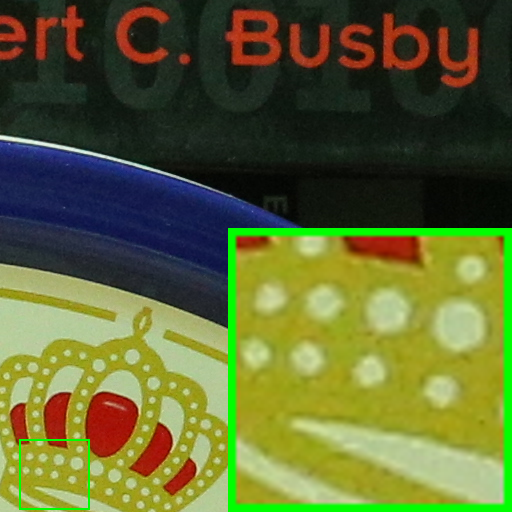
\includegraphics[width=1\textwidth]{images/br_Noisy_5dmark3_iso3200_1.png}}
{\footnotesize (a) Real Noisy Image}
\end{minipage}
\begin{minipage}[t]{0.2\textwidth}
\centering
\raisebox{-0.15cm}{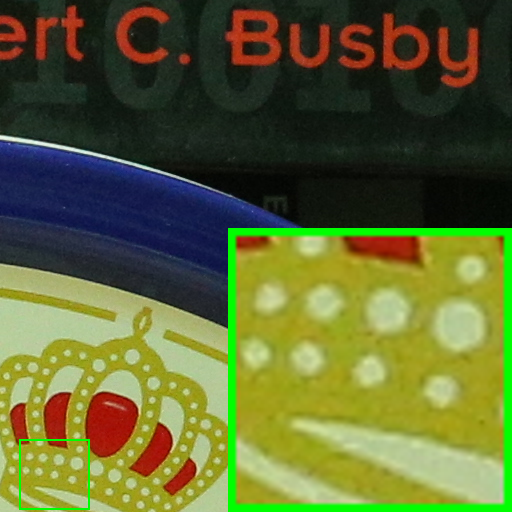
\includegraphics[width=1\textwidth]{images/br_BM3D_5dmark3_iso3200_1.png}}
{\footnotesize (b) BM3D}
\end{minipage}
\begin{minipage}[t]{0.2\textwidth}
\centering
\raisebox{-0.15cm}{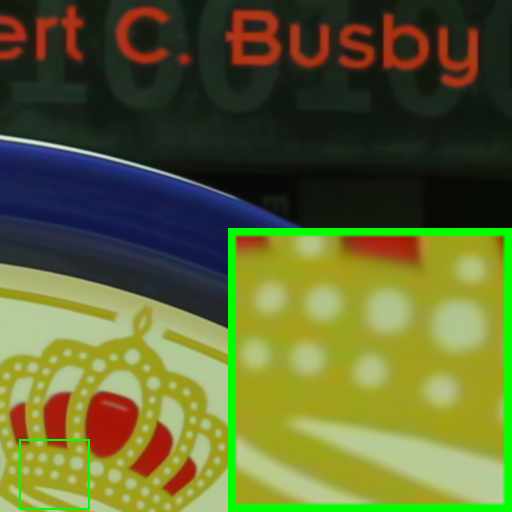
\includegraphics[width=1\textwidth]{images/br_WNNM_5dmark3_iso3200_1.png}}
{\footnotesize (c) WNNM}
\end{minipage}
\begin{minipage}[t]{0.2\textwidth}
\centering
\raisebox{-0.15cm}{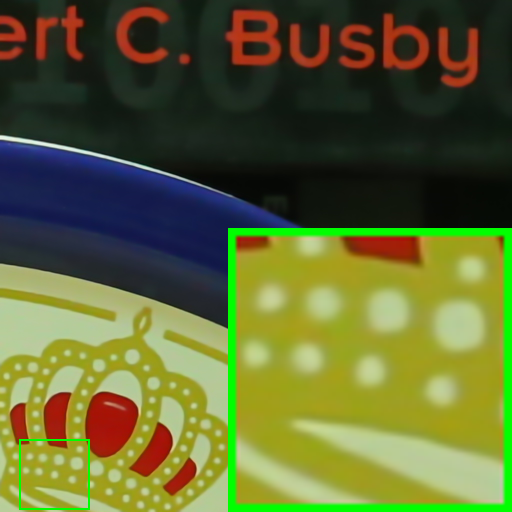
\includegraphics[width=1\textwidth]{images/br_CSF_5dmark3_iso3200_1.png}}
{\footnotesize (d) CSF}
\end{minipage}
\begin{minipage}[t]{0.2\textwidth}
\centering
\raisebox{-0.15cm}{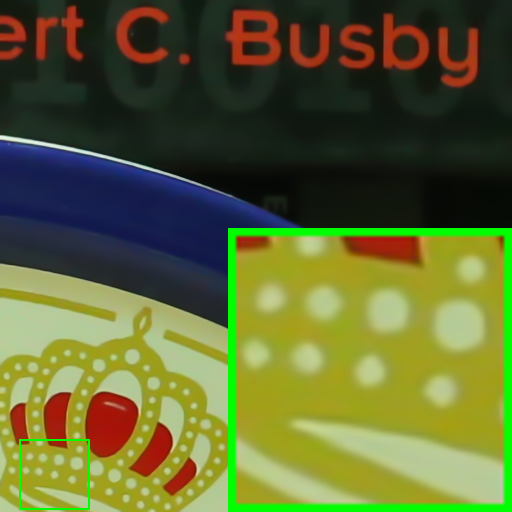
\includegraphics[width=1\textwidth]{images/br_TRD_5dmark3_iso3200_1.png}}
{\footnotesize (e) TRD}
\end{minipage}
}
\subfigure{
\begin{minipage}[t]{0.2\textwidth}
\centering
\raisebox{-0.15cm}{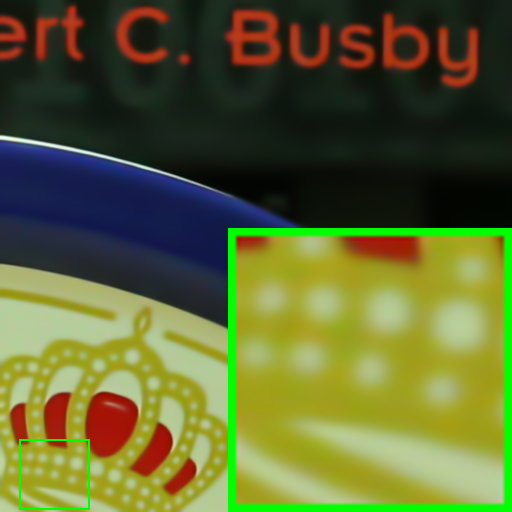
\includegraphics[width=1\textwidth]{images/br_MLP_5dmark3_iso3200_1.png}}
{\footnotesize (f) MLP}
\end{minipage}
\begin{minipage}[t]{0.2\textwidth}
\centering
\raisebox{-0.15cm}{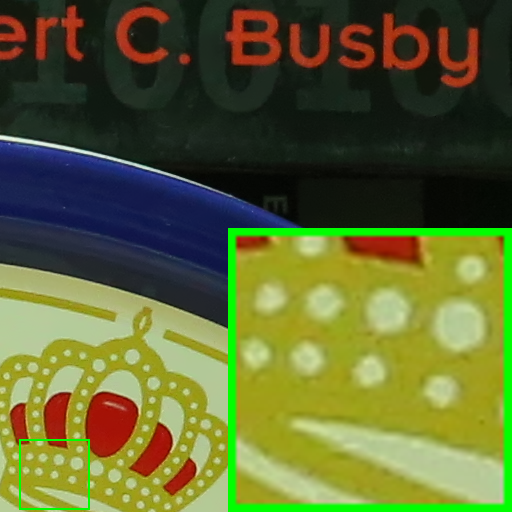
\includegraphics[width=1\textwidth]{images/br_NC_5dmark3_iso3200_1.png}}
{\footnotesize (g) Noise Clinic}
\end{minipage}
\begin{minipage}[t]{0.2\textwidth}
\centering
\raisebox{-0.15cm}{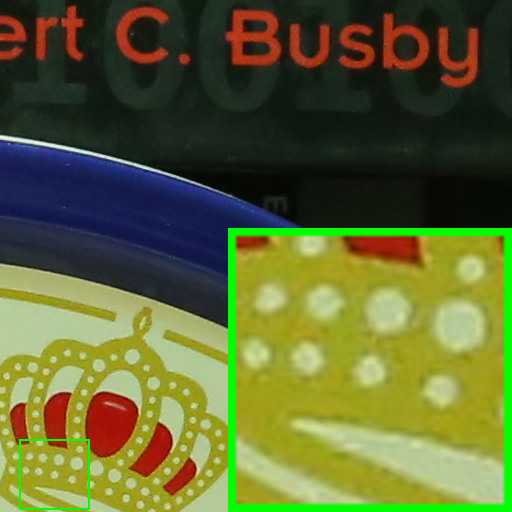
\includegraphics[width=1\textwidth]{images/br_NI_5dmark3_iso3200_1.png}}
{\footnotesize (h) Neat Image}
\end{minipage}
\begin{minipage}[t]{0.2\textwidth}
\centering
\raisebox{-0.15cm}{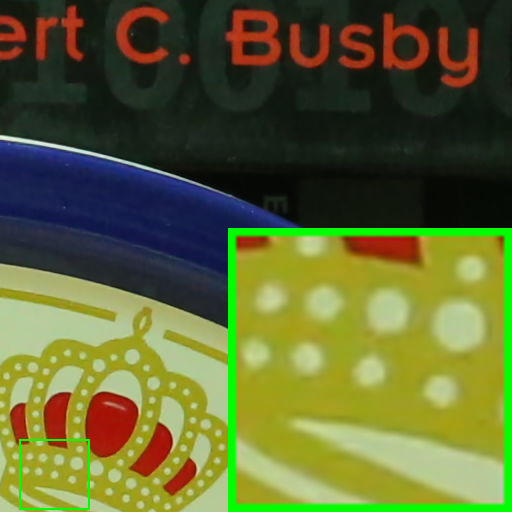
\includegraphics[width=1\textwidth]{images/br_DSCDL_5dmark3_iso3200_1.png}}
{\footnotesize (i) Ours }
\end{minipage}
\begin{minipage}[t]{0.2\textwidth}
\centering
\raisebox{-0.15cm}{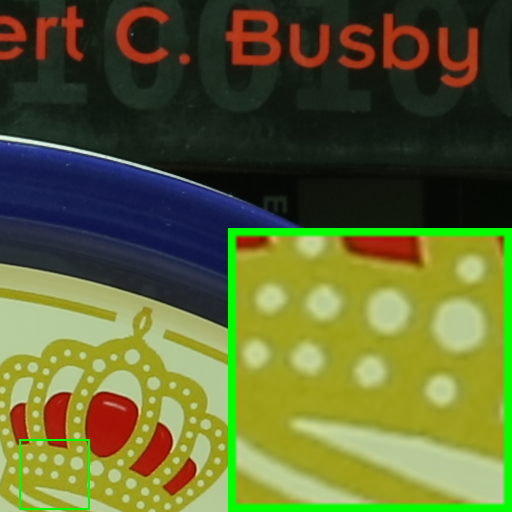
\includegraphics[width=1\textwidth]{images/br_Mean_5dmark3_iso3200_1.png}}
{\footnotesize (j) Mean Image }
\end{minipage}
}
\caption{Denoised images of the old image "$5dmark3_iso3200_1$" by different methods. The images are better to be zoomed in on screen.}
\label{fig2}
\end{figure*}

\begin{figure*}
\centering
\subfigure{
\begin{minipage}[t]{0.2\textwidth}
\centering
\raisebox{-0.15cm}{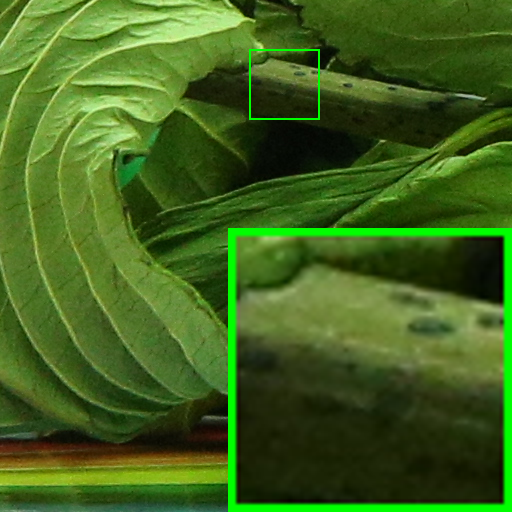
\includegraphics[width=1\textwidth]{images/br_Noisy_5dmark3_iso3200_2.png}}
{\footnotesize (a) Real Noisy Image}
\end{minipage}
\begin{minipage}[t]{0.2\textwidth}
\centering
\raisebox{-0.15cm}{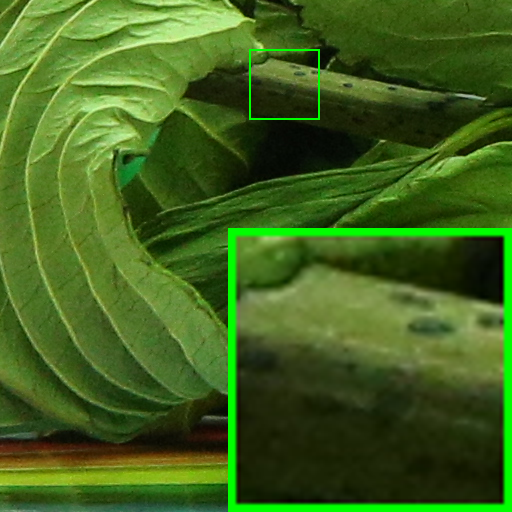
\includegraphics[width=1\textwidth]{images/br_BM3D_5dmark3_iso3200_2.png}}
{\footnotesize (b) BM3D}
\end{minipage}
\begin{minipage}[t]{0.2\textwidth}
\centering
\raisebox{-0.15cm}{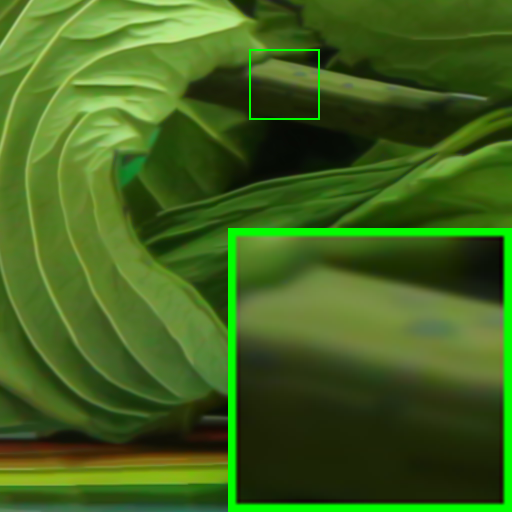
\includegraphics[width=1\textwidth]{images/br_WNNM_5dmark3_iso3200_2.png}}
{\footnotesize (c) WNNM}
\end{minipage}
\begin{minipage}[t]{0.2\textwidth}
\centering
\raisebox{-0.15cm}{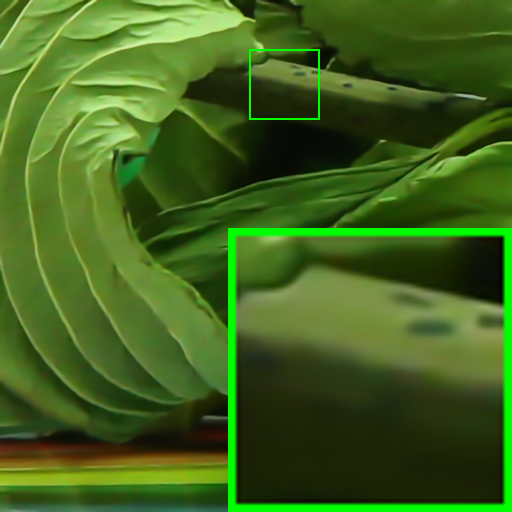
\includegraphics[width=1\textwidth]{images/br_CSF_5dmark3_iso3200_2.png}}
{\footnotesize (d) CSF}
\end{minipage}
\begin{minipage}[t]{0.2\textwidth}
\centering
\raisebox{-0.15cm}{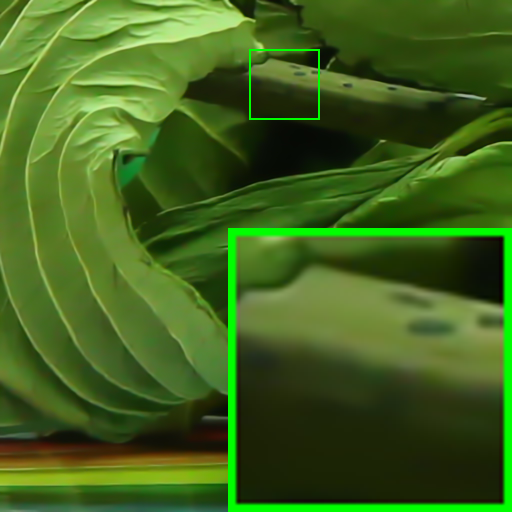
\includegraphics[width=1\textwidth]{images/br_TRD_5dmark3_iso3200_2.png}}
{\footnotesize (e) TRD}
\end{minipage}
}
\subfigure{
\begin{minipage}[t]{0.2\textwidth}
\centering
\raisebox{-0.15cm}{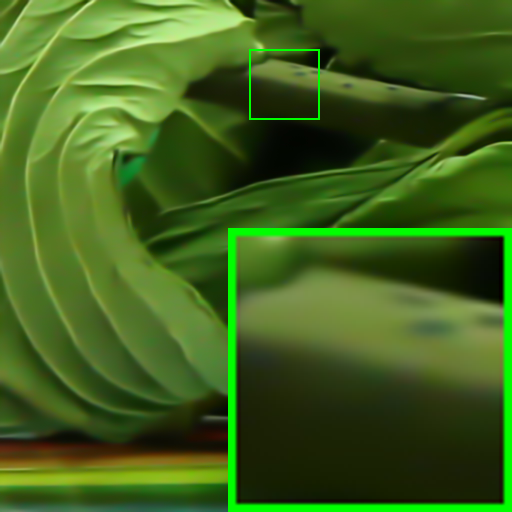
\includegraphics[width=1\textwidth]{images/br_MLP_5dmark3_iso3200_2.png}}
{\footnotesize (f) MLP}
\end{minipage}
\begin{minipage}[t]{0.2\textwidth}
\centering
\raisebox{-0.15cm}{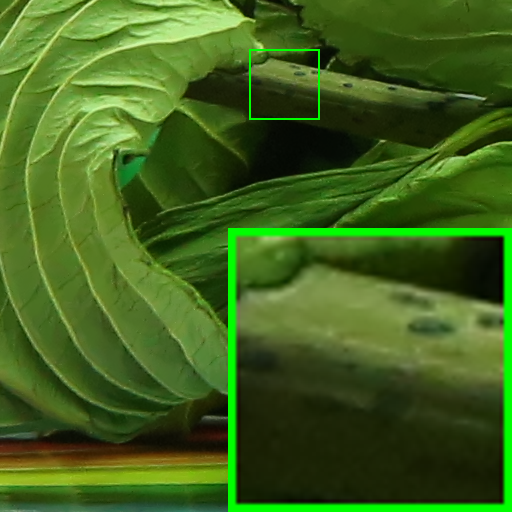
\includegraphics[width=1\textwidth]{images/br_NC_5dmark3_iso3200_2.png}}
{\footnotesize (g) Noise Clinic}
\end{minipage}
\begin{minipage}[t]{0.2\textwidth}
\centering
\raisebox{-0.15cm}{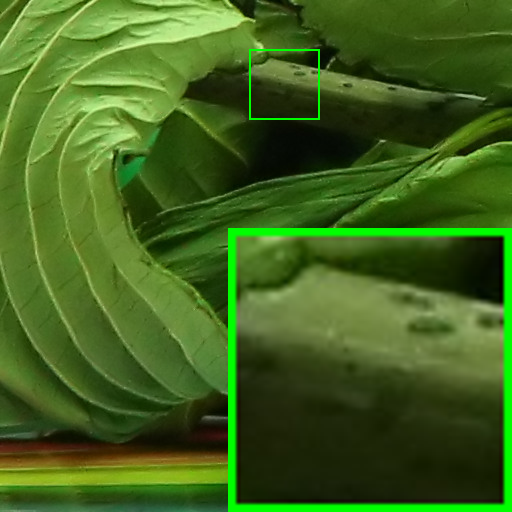
\includegraphics[width=1\textwidth]{images/br_NI_5dmark3_iso3200_2.png}}
{\footnotesize (h) Neat Image}
\end{minipage}
\begin{minipage}[t]{0.2\textwidth}
\centering
\raisebox{-0.15cm}{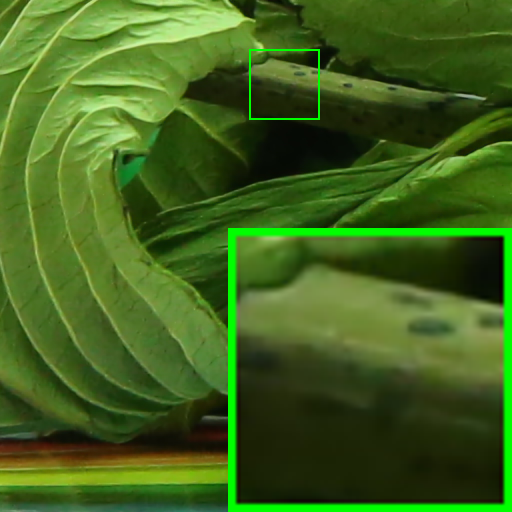
\includegraphics[width=1\textwidth]{images/br_DSCDL_5dmark3_iso3200_2.png}}
{\footnotesize (i) Ours }
\end{minipage}
\begin{minipage}[t]{0.2\textwidth}
\centering
\raisebox{-0.15cm}{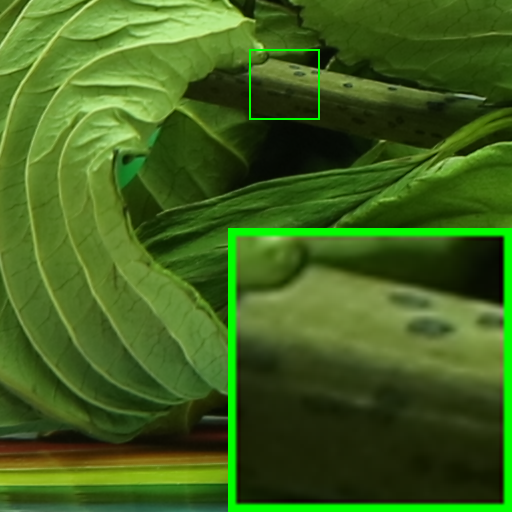
\includegraphics[width=1\textwidth]{images/br_Mean_5dmark3_iso3200_2.png}}
{\footnotesize (j) Mean Image }
\end{minipage}
}
\caption{Denoised images of the old image "$5dmark3_iso3200_2$" by different methods. The images are better to be zoomed in on screen.}
\label{fig2}
\end{figure*}


\begin{figure*}
\centering
\subfigure{
\begin{minipage}[t]{0.2\textwidth}
\centering
\raisebox{-0.15cm}{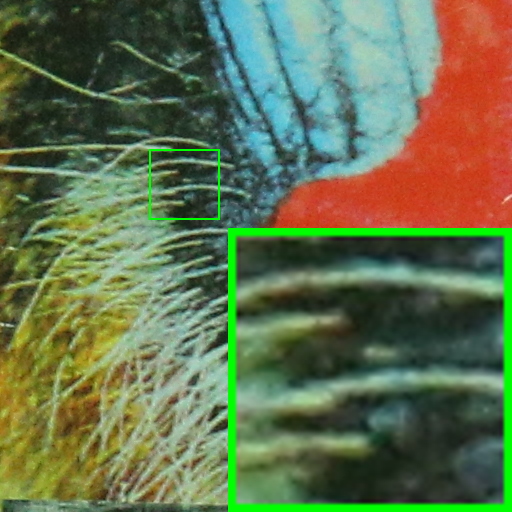
\includegraphics[width=1\textwidth]{images/br_Noisy_5dmark3_iso3200_3.png}}
{\footnotesize (a) Real Noisy Image}
\end{minipage}
\begin{minipage}[t]{0.2\textwidth}
\centering
\raisebox{-0.15cm}{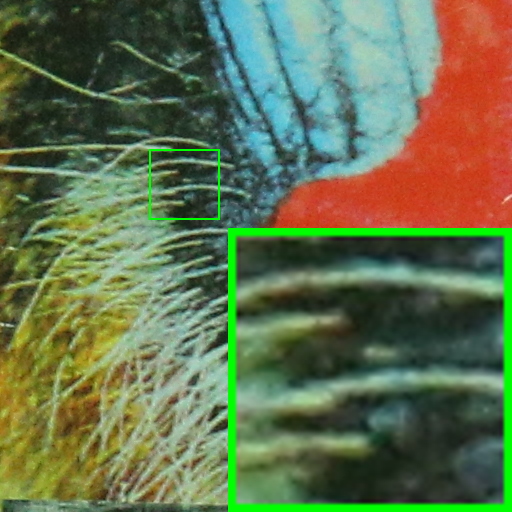
\includegraphics[width=1\textwidth]{images/br_BM3D_5dmark3_iso3200_3.png}}
{\footnotesize (b) BM3D}
\end{minipage}
\begin{minipage}[t]{0.2\textwidth}
\centering
\raisebox{-0.15cm}{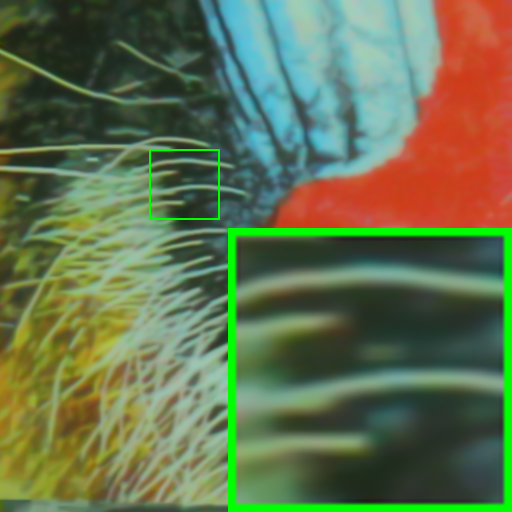
\includegraphics[width=1\textwidth]{images/br_WNNM_5dmark3_iso3200_3.png}}
{\footnotesize (c) WNNM}
\end{minipage}
\begin{minipage}[t]{0.2\textwidth}
\centering
\raisebox{-0.15cm}{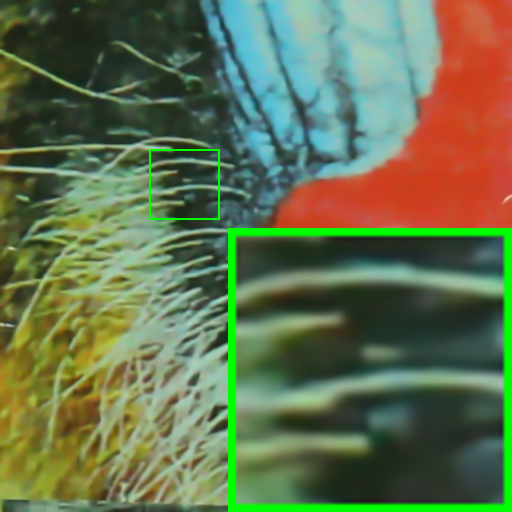
\includegraphics[width=1\textwidth]{images/br_CSF_5dmark3_iso3200_3.png}}
{\footnotesize (d) CSF}
\end{minipage}
\begin{minipage}[t]{0.2\textwidth}
\centering
\raisebox{-0.15cm}{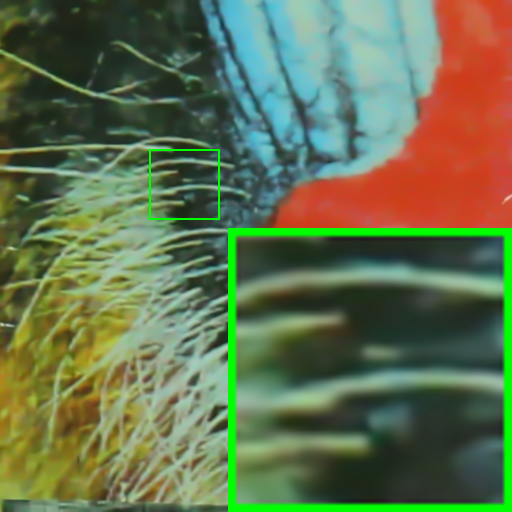
\includegraphics[width=1\textwidth]{images/br_TRD_5dmark3_iso3200_3.png}}
{\footnotesize (e) TRD}
\end{minipage}
}
\subfigure{
\begin{minipage}[t]{0.2\textwidth}
\centering
\raisebox{-0.15cm}{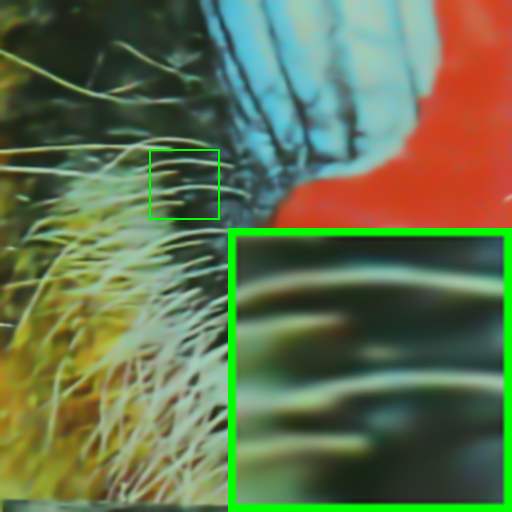
\includegraphics[width=1\textwidth]{images/br_MLP_5dmark3_iso3200_3.png}}
{\footnotesize (f) MLP}
\end{minipage}
\begin{minipage}[t]{0.2\textwidth}
\centering
\raisebox{-0.15cm}{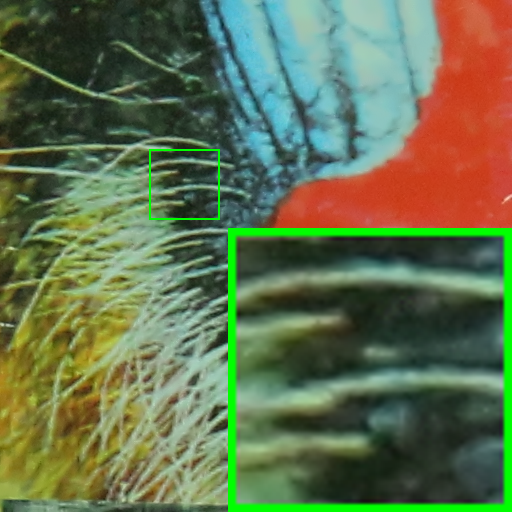
\includegraphics[width=1\textwidth]{images/br_NC_5dmark3_iso3200_3.png}}
{\footnotesize (g) Noise Clinic}
\end{minipage}
\begin{minipage}[t]{0.2\textwidth}
\centering
\raisebox{-0.15cm}{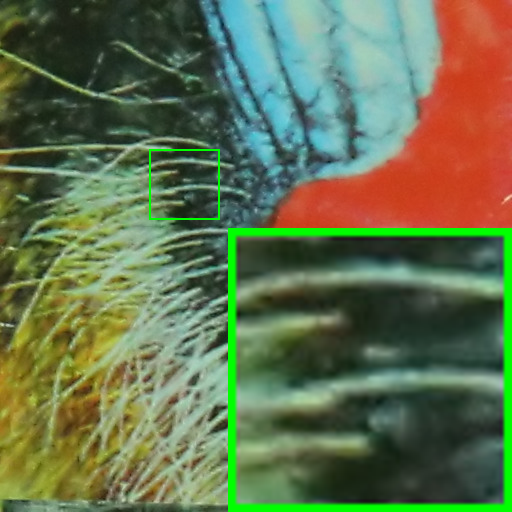
\includegraphics[width=1\textwidth]{images/br_NI_5dmark3_iso3200_3.png}}
{\footnotesize (h) Neat Image}
\end{minipage}
\begin{minipage}[t]{0.2\textwidth}
\centering
\raisebox{-0.15cm}{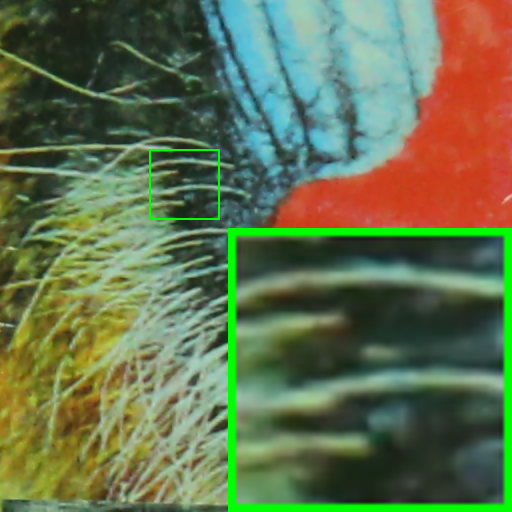
\includegraphics[width=1\textwidth]{images/br_DSCDL_5dmark3_iso3200_3.png}}
{\footnotesize (i) Ours }
\end{minipage}
\begin{minipage}[t]{0.2\textwidth}
\centering
\raisebox{-0.15cm}{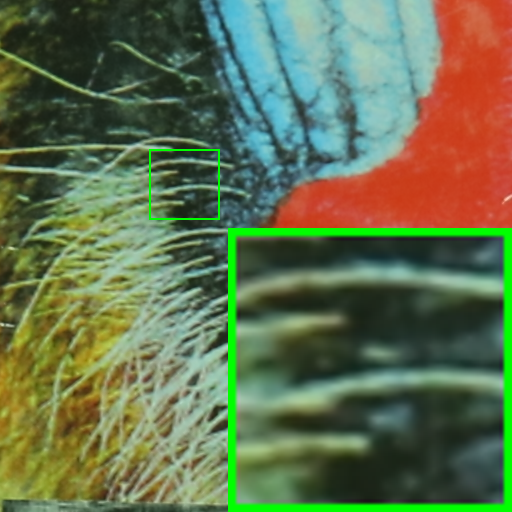
\includegraphics[width=1\textwidth]{images/br_Mean_5dmark3_iso3200_3.png}}
{\footnotesize (j) Mean Image }
\end{minipage}
}
\caption{Denoised images of the old image "$5dmark3_iso3200_3$" by different methods. The images are better to be zoomed in on screen.}
\label{fig2}
\end{figure*}



\begin{table*}
\caption{Average PSNR(dB) and SSIM results of different methods on 42 cropped images from 17 real noisy images in \cite{crosschannel2016}.}
\label{tab1}
\begin{center}
\renewcommand\arraystretch{1}
\begin{tabular}{|c||c|c|c|c|c|c|c|c|c|c|}
\hline
Measure & \textbf{Noisy} &\textbf{BM3D}&\textbf{WNNM}&\textbf{CSF}&\textbf{TRD}&\textbf{MLP}& \textbf{Noise Clinic}& \textbf{Neat Image}&\textbf{Ours}
\\
\hline
PSNR& 34.36 & 34.36 & 34.40 & 36.11 & 36.05 & 34.41 & 37.68 & 36.58 & 36.15
\\
\hline
SSIM& 0.8552 & 0.8553 & 0.8577 & 0.9215 & 0.9211 & 0.9012 & 0.9470 & 0.9145 & 0.9236
\\
\hline
\end{tabular}
\end{center}
\end{table*}


\section{Conclusion and Future Work}

In the future, we will evaluate the proposed method on other conputer vision tasks such as single image super-resolution, photo-sketch synthesis, and cross-domain image recognition. Our proposed method can be improved if we use better training images, fine tune the parameters via cross-validation. We believe that our framework can be useful not just for real image denoising, but for image super-resolution, image cross-style synthesis, and recognition tasks. This will be our line of future work.

{\small
\bibliographystyle{unsrt}
\bibliography{egbib}
}

\end{document}
